%\documentclass[DIV=calc,paper=a4,fontsize=11pt, onecolumn, oneside]{scrartcl}	 					
%\usepackage[english]{babel}

\documentclass[11pt,a4paper]{article}
\usepackage[latin1]{inputenc}
\usepackage{amsmath}
\usepackage{amsfonts}
\usepackage{float}
\usepackage{graphicx}
\usepackage{fullpage}
\usepackage{caption}
\usepackage{subfig}
\usepackage[parfill]{parskip}
\usepackage{footnote}




%%% NOTE! XeLaTeX necessary! %%%
%%% MARGINS %%%
\usepackage{fullpage}
\usepackage[a4paper, margin=1in]{geometry}
\usepackage{setspace}
\usepackage{multicol}

%%% GRAPHICS %%%
\usepackage{graphicx}
\usepackage{color}
\usepackage{graphics}
\usepackage{microtype}
\usepackage{rotating}
\usepackage{subfig}
\usepackage{amsmath}
\usepackage{amssymb}
\usepackage{amscd}
%\usepackage{xfrac}
%\usepackage{dsfont}



\author{Louis Dijkstra\footnote{\textbf{Student no. VU:} 2513226 \textbar\ \textbf{E-mail:} \texttt{Louis.Dijkstra@student.uva.nl}} \ \ \ \ \ Jeroen Hofman\footnote{\textbf{Student no. VU:} 2513225 \textbar\ \textbf{E-mail:} \texttt{Jeroen.Hofman@student.uva.nl}} \ \ \ \ \ Daniel Karavolos\footnote{\textbf{Student no. VU:} 2510702 \textbar\ \textbf{E-mail:} \texttt{Daniel.Karavolos@student.uva.nl}}  \\[15pt] University of Amsterdam (\textsc{UvA})}

\title{The Effect of Fish Schooling on Predation\\
		}


\begin{document}
\captionsetup{width=0.8\textwidth}
\maketitle

\begin{abstract}
\noindent\small{ We extended the model for the formation of fish schools introduced by Hemelrijk et. al. (2008) by adding a predator to the environment. Fish are thought to form schools in order to protect themselves from predators. We tested whether the forming of a school in this model might indeed be beneficial by testing how long it takes for the predator to eat the fish. We found that it takes the predator a longer time to catch all the fish when the fish swim in a random fashion rather than in a school. This result is consistent for different parameter settings. Therefore we conclude that, in this model, the fish do not benefit from swimming in a school. This is most likely caused by unrealistic modeling of the predator.  \\[10pt]
\noindent \textbf{Keywords:} \textbullet\ Fish school \ \textbullet\ Predation \ \textbullet\ 3 Dimensional Model }
\end{abstract}

\newpage
\tableofcontents
\newpage

\section{Introduction}
\label{sec:intro}
%The effect of fish schools on the successfulness of predators has long been a subject of scientific research. Since there are many different types of fish schools and predators, there are many publications about the behavior of specific species. 
There have been many models on flocking behavior of animals. Arguably the most famous of these is Craig Reynolds' boids model \cite{reynolds}. Most of the models focus on flocking patterns in two dimensions, but since the current generation of computers made it possible to handle the computations for these models in 3D, there has been a shift of focus towards these more realistic 3D models.

In 2008 Hemelrijk et al. \cite{hemelrijk} presented a 3D extension of their 2D model of fish schools. They showed that the individual rules %and forces?
that facilitate the emergent pattern of schooling in fish in 2D can be extended to 3D rules. Furthermore, they showed that these rules not only account for the emergence of schooling, but also for the oblong shape that is found in real fish schools. 
There is evidence that swimming in schools has certain hydrodynamic advantages \cite{svendsen}. We are, however, more interested whether swimming in a school results in a higher chance of survival \cite{cullen}. 

In this report we present a very general model of predator/prey behavior, based on the 3D fish school model of Hemelrijk et al. \cite{hemelrijk}. There has been some research on the evolution of prey strategies in a similar setting \cite{kunz06}. This differs from our research in the sense that the strategies of our individuals are fixed in each situation and that our prey are able to sense the predator and flee away from it.

The main goal of our research is to investigate whether schooling among fish helps to protect them from predators in this model. We hypothesize that this is the case and we will test this for varying population sizes and predator speeds. In our model there is only one predator, so that we do not have to take cooperative hunting behavior into account.

In the next section we will present the model and in section \ref{sec:impl} we will describe our implementation. Section \ref{sec:exp} will describe our experimental setup, which is followed by our results in section 5. Finally, we will discuss the results and present our conclusions in section 6.

\section{Model}
\label{sec:model}
%Forces description
%Formulas
\subsection{Perception Zones}
Fish in a school react differently to each other depending on the distance between them, hence there is the need for a certain model which describes these different types of perception. In the model we use a perception model of the fish consisting of three different behavioral zones which can also be found in figure \ref{fig:perczones}:
\begin{itemize}
\item 
  \textbf{Separation zone}: This is a small zone around an individual where it tries to avoid any other individuals in that zone. Individuals use both their vision and their lateral line system  so they have a fairly large viewing angle (much broader than humans). Only a small area behind the fish is usually excluded from this zone.
\item
  \textbf{Alignment zone}: This is a larger zone than the separation zone (excluding the separation zone itself), in which the individual tries to align with other individuals in that zone, using its lateral line system \cite{hemelrijk}. Since it depends on the lateral line system of the fish, parts at the back and the front of the fish are excluded from the zone.
\item
  \textbf{Cohesion zone}: This is the largest zone, excluding both the separation zone and the alignment zone. Every individual is attracted to the other fish in this zone. The perception in this zone is mere visual, so a portion at the back of the fish is excluded.
\end{itemize}

\begin{figure}[H]
  \centering
  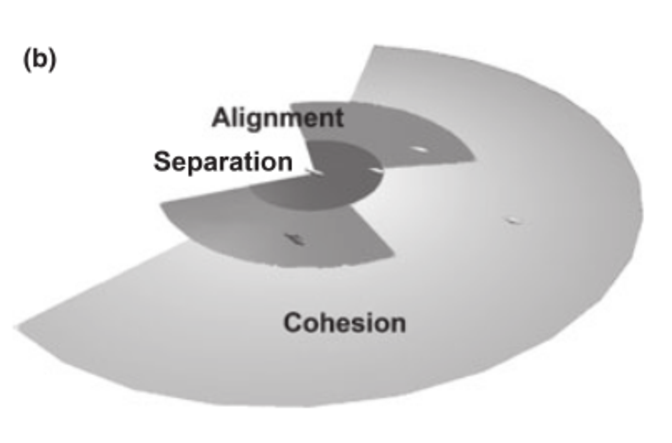
\includegraphics{perczones.pdf}
  \caption{Two dimensional view of the fish perception zones. The figure is taken from \cite{hemelrijk}. We use another definition for the cohesion zone (see text).}
  \label{fig:perczones}
\end{figure}

In order to simulate local perception, Hemelrijk et al. proposed to adapt the radii of the alignment and cohesion zone every time step according to the total number of perceivable fish in the associated zones (the radius of the separation zone is fixed and set to $R_{\text{min}}$). The rationale behind this flexible range of perception is that when the number of neighboring fish in- or decreases, fish, that are further away, are more/less visible. 

The adaption of the fish range of perception, $R_i$, is performed as follows:
\begin{equation}
R_i(t + \Delta t) = \text{max} \left\{ R_{\text{min}}, R_i(t)(1 - n_i \Delta t (R_{\text{max}} - n_w n(t) + 1) \right\}
\label{eq:R}
\end{equation}
where $R_i(t + \Delta t)$ is the radius of perception at time step $(t + \Delta t)$, $n(t)$ is the number of neighbors in the cohesion zone at time $t$, $n_w$ indicates the influence of one single neighbor and $0 \leq n_i \leq 1$ controls the smoothness of the radius adaptation, i.e., if $n_i$ is equal to $1$, the radius is adapted instantly to the current number of neighbors in the respective perception zone of the fish. When $n_i$ is $0$, the radius stays constant. 


\subsection{Forces}
The movement of every fish is governed by seven different forces that can be grouped into two categories: interaction and individual forces. Under interaction forces we understand the separation, alignment, cohesion and flee force, since all four of them take the position and/or orientation of the neighboring fish or predator into consideration:
\begin{enumerate}
\item \textbf{Separation force}, $\mathbf{f}_{s}$: in order to avoid collision, fish move away from neighbors in their separation zone. 
\item \textbf{Alignment force}, $\mathbf{f}_{a}$: fish align with the neighbors in their alignment zone. 
\item \textbf{Cohesion force}, $\mathbf{f}_{c}$: fish are drawn to the center of gravity of the school of fish. 
\item \textbf{Flee force}, $\mathbf{f}_{\text{flee}}$: fish flee from the position of the predator. 
\end{enumerate}
The three individual forces are:
\begin{enumerate}
\setcounter{enumi}{4}
\item \textbf{Correctional speed force}, $\mathbf{f}_{\text{speed}}$: every fish tries to swim at its desired velocity, $v0$. 
\item \textbf{Correctional pitch force}, $\mathbf{f}_{p}$: fish normally do not show large pitch angles (they tend not to swim downward or upward \cite{hemelrijk}). This force reduces the pitch angle fish might have. 
\item \textbf{Random force}, $\mathbf{f}_\text{random}$: a random force is added to account for imperfect decision-making and noise in the environment. 
\end{enumerate}
All these forces together form the net force:
\begin{equation}
\mathbf{f}_\text{net} = \mathbf{f}_s + \mathbf{f}_a + \mathbf{f}_c + \mathbf{f}_\text{flee} + \mathbf{f}_\text{speed} + \mathbf{f}_p + \mathbf{f}_\text{random}
\label{eq:fnet}
\end{equation}
which is rescaled to $3$, if the net force is larger than $3$.

We will describe each of the forces in the sections \ref{sec:interactionF} (interaction forces) and \ref{sec:non-interaction} (individual forces). 

\subsubsection{Interaction Forces} \label{sec:interactionF}
In order to avoid collision with the fish in the separation zone, every fish experiences a separation force pointed in the opposite direction of the weighted average of the directions of the neighboring fish. In order to compute this force, we compute $\mathbf{r}_j - \mathbf{r}_i$ for every fish $j$ in the separation zone of the fish $i$ (the fish currently under consideration). 
 
The weighted average direction of the neighbors in the separation zone is defined as
$$
\mathbf{d}_{s,i} = \frac{1}{n_s} \displaystyle\sum\limits_{j = 1}^{n_s} \frac{\mathbf{r}_j - \mathbf{r}_i}{\left|\mathbf{r}_j - \mathbf{r}_i\right|^2}
$$
where $n_s$ is the number of fish in the separation zone of fish $i$ and $|\cdot|$ denotes the norm.  
The separation force is then defined as follows:
\begin{equation}
\mathbf{f}_{s,i} = - w_s \frac{\mathbf{d}_{s,i}}{\left| \mathbf{d}_{s,i} \right|} \cdot 
\label{eq:fs}
\end{equation}
where $w_s$ is a parameter, referred to as the separation weight.

The fish also perceives an alignment force, that steers its orientation towards the average directions of the surrounding fish in its alignment zone. The average orientation is defined as
$$
\mathbf{d}_{a, i} = \frac{1}{n_a} \displaystyle\sum\limits_{j = 1}^{n_a} \mathbf{e}_{f,j}
$$
where $n_a$ is the number of neighbors in the alignment zone of fish $i$ and $\mathbf{e}_{f,j}$ is the forward orientation of fish $j$. The alignment force then becomes
\begin{equation}
\mathbf{f}_{a,i} = - w_a \frac{\mathbf{d}_{a,i} - \mathbf{e}_{f,i}}{\left|\mathbf{d}_{a,i} - \mathbf{e}_{f,i} \right|}
\label{eq:fa}
\end{equation}
where $w_a$ is a parameter, referred to as the alignment weight.

Fish are attracted to the center of mass of the school. We compute
$$
\mathbf{d}_{c,i} = \frac{1}{N} \displaystyle\sum\limits_{j = 1}^{N} \frac{\mathbf{r}_j - \mathbf{r}_i}{\left|\mathbf{r}_j - \mathbf{r}_i\right|}
$$
where $N$ is the total number of fish in the environment. We define the cohesion force, $\mathbf{f}_c$, as
\begin{equation}
\mathbf{f}_c = w_c \frac{\mathbf{d}_{c,i}}{\left|\mathbf{d}_{c,i} \right|}
\label{eq:fc}
\end{equation}
where $w_c$ is a parameter, referred to as the cohesion weight. 

The cohesion force is, in contrast to the original model introduced by Hemelrijk et al. (2008), not locally defined, in the sense that in our implementation of this force, the positions of all fish in the environment are taken into account. This is of course not so realistic, but makes sure that, when under attack by a predator, the school of fish does not suddenly fall apart into smaller groups, which was the case when we used the same definition as Hemelrijk et al. (2008). 

The fourth and last interaction force, is the result of interaction between the fish and the predator. As expected, the fish try to get away as far as possible from the predators position, $\mathbf{r}_\text{predator}$, at all cost, while the predator tries to devour as much fish as it possibly can.  

The flee force for fish $i$ is defined as
\begin{equation}
\mathbf{f}_{\text{flee}, i} = - w_\text{flee} \frac{\mathbf{r}_\text{predator} - \mathbf{r}_i}{\left|\mathbf{r}_\text{predator} - \mathbf{r}_i\right|}
\label{eq:flee}
\end{equation}
where $w_\text{flee}$ is a parameter, $\mathbf{r}_\text{predator}$ is the current position of the predator and $\mathbf{r}_i$ is the position of fish $i$.In words, the closer the fish get to the predator, the larger the flee force becomes. 

Note that the magnitude of all these interaction forces are governed by their associated parameters ($w_s$, $w_a$, $w_c$ and $w_\text{flee}$) and, hence, these parameters denote the relative influence on the net force (see equation \ref{eq:fnet}).  
 
\subsubsection{Individual Forces} \label{sec:non-interaction}
In addition to interaction forces, every fish is influenced by three other individual forces: a correctional speed force, $\mathbf{f}_{\text{speed}, i}$, a correctional pitch force, $\mathbf{f}_{p,i}$, and a random force, $\mathbf{f}_\text{random}$. 

The correctional speed force, $\mathbf{f}_{\text{speed}, i}$, forces the fish to return to its desired/default velocity, $v_0$. The force is defined as 
\begin{equation}
\mathbf{f}_{\text{speed}, i} = \frac{v_0 - |\mathbf{v}_i|}{\tau} \mathbf{e}_{f,i}
\label{eq:fspeed}
\end{equation}
where $v_0$ is the desired velocity, $|\mathbf{v}_i|$ is the magnitude of the velocity vector, $\tau$ is the 'relaxation time' introduced to make sure the speed of a fish is not updated instantly and $\mathbf{e}_{f,i}$ is the forward direction of fish $i$. 

The correctional pitch force returns fish to their natural horizontal position. The force is defined as
\begin{equation}
\mathbf{f}_{p, i} = \begin{pmatrix}0 \\ 0 \\ -w_{pc} \cdot e_z \end{pmatrix}
\label{eq:fp}
\end{equation}
where $e_z$ is the $z$-element of the forward direction vector $\mathbf{e}_{f,i}$ and $w_{pc}$ is a parameter, referred to as the correctional pitch weight. 

We also introduce a random force in order to account for imperfect decision-making and a noisy environment. The random force, $\mathbf{f}_{\text{random},i}$, is a randomly generated vector with a maximum predefined magnitude. 

\subsection{Predator} 
% Behavior predator
The predator is defined by its position in the three dimensional environment, $\mathbf{r}_\text{predator}$, the speed of the predator, $v_\text{predator}$, and, what we refer to as, the relaxation time, $t_\text{relax}$. This relaxation time denotes the interval the predator needs after it caught a fish, before it can catch another one. 

The behavior of the predator is simple; it moves with a constant speed to the nearest fish in its vicinity. Which fish is the closest is determined every single iteration step. This might cause the predator to be 'confused' (i.e., it might have to change its direction often). 
Which fish is closest to the predators position is determined by
$$
\mathbf{r}_\text{closest} = \operatorname*{min}_{i} |\mathbf{r}_\text{predator} - \mathbf{r}_i|
$$
where $\mathbf{r}_{i}$ is the current position of fish $i$. The position of the predator is adapted as follows
\begin{equation}
\mathbf{r}_\text{predator}(t + \Delta t) = \mathbf{r}_\text{predator}(t) + v_\text{predator} \Delta t \frac{\mathbf{r}_\text{closest} - \mathbf{r}_\text{predator}(t)}{\left|\mathbf{r}_\text{closest} - \mathbf{r}_\text{predator}(t) \right|}
\label{eq:fpredator}
\end{equation}

When a fish is in the circle with a certain predefined radius, $R_\text{eat}$, around the predator, it is considered eaten. We remove the fish from the environment. The predator cannot devour any more fish until the end of its predefined relaxation time, $t_\text{relax}$. 



\section{Implementation}
\label{sec:impl}
%Perception zone
%Model (JAVA/MASON)

\subsection{Perception zones}
For the implementation of the perception zones we have to create an algorithm with which we can decide whether a fish is in one of the perception zones of some individual, described in the section \ref{sec:model}. As explained before there are three perception zones of the fish: the cohesion zone, the alignment zone and the separation zone. The separation and alignment zone are implemented as in \cite{hemelrijk}. As mentioned before, we use an adaptation of the cohesion zone, i.e., the cohesion zone is the entire environment. 
In the model we have to check for every fish how many neighbors there are in these zones in order to compute the forces in equations \ref{eq:fs}, \ref{eq:fa} and \ref{eq:fc}. The three different zones for a fish are shown in figure \ref{fig:perczones}. The figure shows three circles where parts are cut out to accommodate the fact that fish cannot see certain parts behind them (in the case of the separation zone) and that alignment only takes place with fish which are in the region perpendicular to the forward direction of the individual considered. While this figure looks relatively simple, there are two properties which make this perception model complicated:

\begin{itemize}
\item 
  Figure \ref{fig:perczones} shown below is two-dimensional, while our model is in three dimensions, so one has to imagine the forms to be spherical instead of circular, which complicates the part of cutting out regions of the spheres where the fish cannot perceive.
\item
  The whole structure rotates in accordance to the forward direction of the fish.
\end{itemize}

We developed an algorithm to determine whether a fish is in the three-dimensional perception zones of an individual, by only taking into account the current forward direction of the individual. Figure \ref{fig:geometry} below shows all the computed quantities graphically. The algorithm consists of the following steps:

\begin{itemize}
\item 
  Consider a fish $i$ at position $\mathbf{x}_i$ together with a forward direction $\mathbf{e}_f$ of the fish. First we check for every fish not equal to fish $i$ in the school whether or not this fish is contained in a sphere with radius $R_\text{min}$ or $R_a$ for the separation and alignment perception zones, respectively. If the fish is in one of the perception radii, it might be in the corresponding perception zone of fish $i$ if it is not in an excluded part of the sphere, shown in figure \ref{fig:perczones}. The next steps will be about determining this which regions are excluded.
\item
  Start with the forward direction $\mathbf{e}_f$ of fish $i$ and determine a vector $\mathbf{e}_s$ perpendicular to $\mathbf{e}_f$ with the restriction that $\mathbf{e}_s$ should have a zero $z$-component. $\mathbf{e}_s$ is the side-ward direction of the fish. Note that by setting the $z$-component to zero it is implied there is no roll force and $\mathbf{e_s}$ is unique up to a sign.
\item
  Compute the cross product of $\mathbf{e}_f$ with $\mathbf{e}_s$ to compute a vector $\mathbf{e}_z$, perpendicular to both vectors. This vector is the normal vector of the plane of movement in which fish $i$ is located. The equation of this plane is defined by all points $(x,y,z)$ in $\mathbb{R}^3$ for which $\mathbf{e}_z \cdot (x,y,z) = 0$.
\item
  Next we rotate the forward vector $\mathbf{e}_f$ around $\mathbf{e}_z$ with some angle $\theta$, dependent on which part of sphere we want to cut out. For instance for the separation zone we want to rotate $\mathbf{e}_f$ with $\theta = 2\pi/3$ and $\theta = 4\pi/3$ to obtain two vectors which mark the boundary of the part of the sphere with the separation radius which we want to exclude (these angles are given in table \ref{tab:param}). We do this rotation by using the standard rotation matrix obtained from \cite{rotmatrix}. In the case of the alignment zone we need four of these vectors, but the two vectors on the front side of the fish are the opposite vectors of the two vectors on the backside.
\item
  Next we take the cross product of the these two or four boundary vectors with $\mathbf{e}_z$, to get the normal vector for two or four planes defined by one of the boundary vectors and $\mathbf{e}_z$. Call these normal vectors $\mathbf{y}_{k}$ for $k = 1,2$ for separation or $k = 1,2,3,4$ for alignment.
\item
  Finally we look at the position of some fish $j$ with position $\mathbf{x}_j$ which is in one of the perception radii (checked in the first step) and check whether its position relative to the position of fish $i$ is in one of the excluded regions. We compute:
  \begin{equation}
    \label{eq:condition}
    (\mathbf{x}_j-\mathbf{x}_i) \cdot \mathbf{y}_1 < 0 \; \text{and} \; (\mathbf{x}_j-\mathbf{x}_i) \cdot \mathbf{y}_2 < 0
  \end{equation}
  If both conditions are met fish $j$ is in the excluded region and so should not be included in the force calculations. In the case of alignment the same condition with $\mathbf{y}_3$ and $\mathbf{y}_4$ also needs to be checked.
\end{itemize}

\begin{figure}[H]
  \centering
  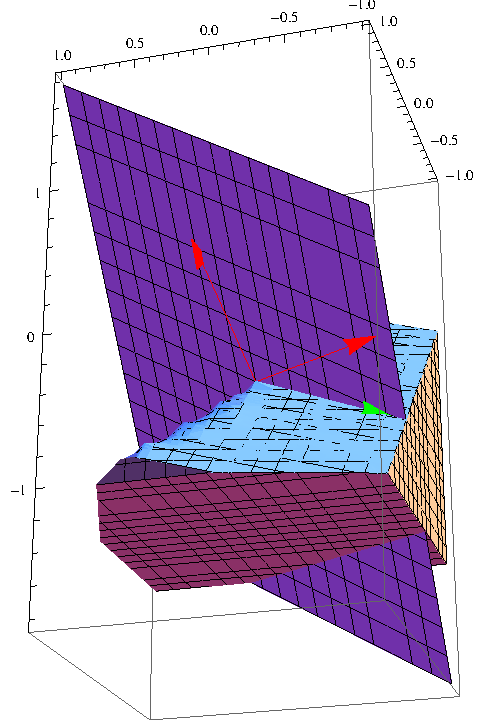
\includegraphics[width=3.0in]{geometry.pdf}
  \caption{Graphical representation of the computed quantities in the steps above. The two red vectors represent $\mathbf{e}_f$ and $\mathbf{e}_s$. The black vector (not clearly visible here) is the normal vector $\mathbf{e}_z$ of the plane going through these two vectors. The green vectors are rotations of $\mathbf{e}_f$ around this normal vector. The region beneath the light blue planes, which are the planes defined by $\mathbf{e}_z$ and a green vector, gives the final excluded region. Note that the normals of the planes going through $\mathbf{e}_z$ and a green vector are not drawn.}
  \label{fig:geometry}
\end{figure}
Fish are assigned random positions in a sphere with a radius of $50$ and the origin as its center. The initial orientations are randomly generated. We start each time step by applying the previous algorithm to all fish in the school. This will gives us the forces on each fish using the force equations from the previous chapter. Then we combine them to compute a net force on the fish according to equation \ref{eq:fnet}. This net force is then converted to a movement by first calculating the acceleration of the fish:
\begin{equation}
  \label{eq:acc}
  \mathbf{a} = \mathbf{f}_\text{net} / m
\end{equation}
and then calculating the new velocity of the fish at the next time step:
\begin{equation}
  \label{eq:vel}
  \mathbf{v}(t + \Delta t) = \mathbf{v}(t) + \mathbf{a} \Delta t
\end{equation}
We can then use this velocity to update the position of fish $i$:
\begin{equation}
  \label{eq:pos}
  \mathbf{r}_i(t + \Delta t) = \mathbf{r}_i(t) + \frac{\Delta t}{2}\left(\mathbf{v}(t) + \mathbf{v}(t + \Delta t)\right)
\end{equation}
where we used a simple quadrature rule for estimating the new position. Every time step we set the forward direction $\mathbf{e}_f$ equal to $\mathbf{v}(t + \Delta t)$ and hence we assume that the fish always head in the direction of movement.

The initial position of the predator is chosen randomly. The predator always starts within a 200 point distance of the origin. 
Every time step we also update the predator position, by calculating which of the fish is the closest one and updating the predators position in the direction of that fish. If the fish comes within the predators radius ($R_\text{eat}$) the fish will be eaten and removed from the environment. After eating the predator has a relaxation time during which it can hunt the next closest fish but it cannot eat it. After the relaxation time the predator will be able to eat the fish again. 

\subsection{Framework}
We have implemented the above mentioned model in Java, using the MASON Toolkit (v.16) \cite{mason} for visualization. Generally it is good practice to separate the model from the visualization and the structure of MASON facilitates that, but it still requires the user to work exactly according to the rules of the framework. Therefore, we choose to implement our model separately from MASON and integrate them after wards. This means that we can run simulations without having to use MASON.

Without MASON our \texttt{main} creates a \texttt{Model}, which contains one predator, called \texttt{predator}, and a \texttt{School} of \texttt{Fish}. The \texttt{Model} keeps track of time and calls the \texttt{update()} of \texttt{School}. The school then updates the positions of all the fish in the school by computing the forces and calling the \texttt{update()} of each individual fish. 
%iets over test?

The visualization of the model (as defined in \texttt{FishSchoolWithUI}) is quite simplistic. The environment is an infinite continuous blue space, in which each fish is represented as a green cone (top up) and the predator %predator?
is a red cone (top sideways), see figure \ref{fig:screen}. We have added a wire frame as a landmark for the viewer. To update the visualization, MASON needs a separate model of the system. The main class should \texttt{extend} the built-in Mason-class \texttt{SimState}, which adds individuals to the environment. And each individual \texttt{implements} the built-in Mason-class \texttt{Steppable}. The individuals are then updated (in terms of behavior) through MASONs \texttt{Scheduler} by calling the overridden \texttt{Step()}-function.

To visualize our simulation, we must synchronize the update-loop of our model with the built-in update-loop (the scheduler) of MASON. Since we shield our implementation from MASON, we do not need the scheduler to update any behavior. We only need it to update the positions of our individuals in the environment. Therefore, the \texttt{step()} of our fish individuals (\texttt{Fish3D}) only consists of checking whether the fish is still alive and retrieving the updated position from the corresponding fish in the model or, when the fish is dead, remove itself from the environment. We have created a \texttt{Steppable SchoolUpdater}, to update the whole school of fish. This class has a \texttt{Model}, of which the \texttt{performOneTimeStep()} is called in each \texttt{step()} of the \texttt{SchoolUpdater}. After that, it calls the \texttt{step()} of each \texttt{Fish3D} in the environment.

Similar to the \texttt{Fish3D}, the \texttt{predator3D} only retrieves the position of the predator %predator?
in the model. It is updated separately from the fish school, but it is always scheduled after the \texttt{SchoolUpdater} so that it always retrieves an updated position from the same time step.

\begin{figure}[t]
\centering
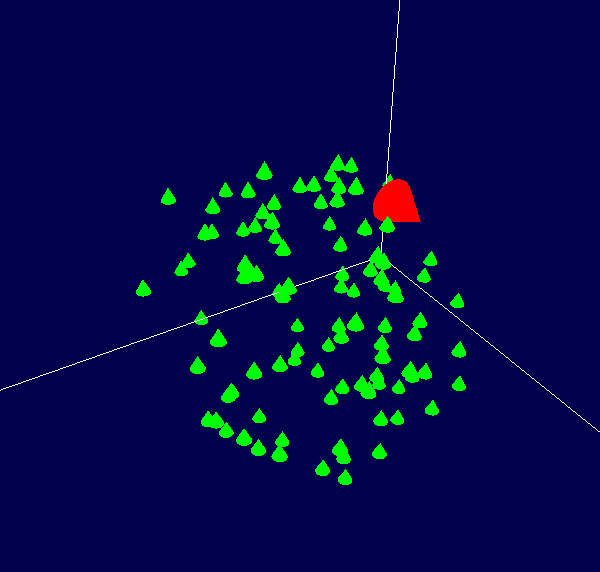
\includegraphics[width = .5\textwidth]{screenshot.png}
\caption{Visualization of the model. The red cone represents the predator, the green cones are the fish.}
\label{fig:screen}
\end{figure}


\section{Experimental set-up}
\label{sec:exp}
%Table parameters
%quantities measured
%Statistics

This model depends on many parameters. We partly use parameter values from \cite{hemelrijk} and partly tweaked the parameters ourselves. Here is a short overview of the parameters we used in our model:

\begin{table}[H]
  \centering
   \caption{Model parameters.}
  \begin{tabular}{l | c | r}
    \hline
    \textbf{Parameter} & \textbf{Symbol} & \textbf{Values}\\
    \hline
    Number of individuals & $N$ & $\left\{2, 7, \ldots, 72, 77 \right\}$\\
    Body mass & - & $1$\\
    Time step & $\Delta t$ & $0.05$\\
    \hline
    \multicolumn{3}{l}{Zone of separation}\\
    \hline
    \; Radius & $R_{\text{min}}$ & $2$\\
    \; Blind angle back & - & $60$\\
    \hline
    \multicolumn{3}{l}{Zone of alignment}\\
    \hline
    \; Maximum radius & - & $5$\\
    \; Blind angle back & - & $60$\\
    \; Blind angle front & - & $60$\\
    \hline
    \multicolumn{3}{l}{Zone of cohesion}\\
    \hline
    \; Maximum radius & - & $15$\\
    \; Blind angle back & - & $90$\\
    \; Cruise speed & $v_0$ & $2$\\
    \hline
    \multicolumn{3}{l}{Weights}\\
    \hline
    \; Separation & $w_s$ & $10$\\
    \; Alignment & $w_a$ & $5$\\
    \; Cohesion & $w_c$ & $9$\\
    \; Flee force & $w_{\text{flee}}$ & $12$\\
    \; Relaxation time & $\tau$ & $0.2$\\
    \; Pitch control & $w_{pc}$ & $2$\\
    \; Random force & $|f_{\text{random}}|$ & $0.5$\\
    \; Max. force & $f_{\text{max}}$ & $3$\\
    \; Neighbor influence & $n_w$ & $1$\\
    \; Smoothness radius adaption & $n_i$ & $0.01$\\
    \hline
    \multicolumn{3}{l}{Predator}\\
    \hline
    \; Eating radius & $R_\text{eat}$ & $2.0$\\
    \; Relaxation time & $t_{\text{relax}}$ & $1.0$, $5.0$\\
    \; Speed & $v_{\text{predator}}$ & $10$, $25$ \\ \hline 
  \end{tabular}
  \label{tab:param}
\end{table}

We allow certain parameters to change in order to test our hypothesis (see table \ref{tab:param}). We vary the number of fish from $2$ up to $77$, the relaxation time of the predator ($1.0$ and $5.0$) and the speed of the predator ($10$ and $25$). We look at two different cases: one, where the fish swim in a school and one, where the fish wander around randomly. The latter is achieved by setting both the alignment and the cohesion force to zero (the separation force is still taking into account, because the fish should not collide). We will look in both cases how long it takes the predator to devour all the fish.  We repeat each experiment 10 times for each fish size to make an error estimate with a 95\% confidence interval defined in the usual way:
\begin{equation}
  \label{eq:error}
  \text{error} = \frac{1.96 \sigma}{\sqrt{10}}
\end{equation}
where $\sigma$ is the sample standard deviation. 

\section{Results}
\label{sec:res}
See figure \ref{fig:results} for the results of our simulations. As you can see, the time the predator needs for catching all the fish is overall larger when the fish swim in a random fashion rather than in schools. This result is consistent for all the parameter settings used. 

\begin{figure}[H]
    \centering
    \subfloat[]{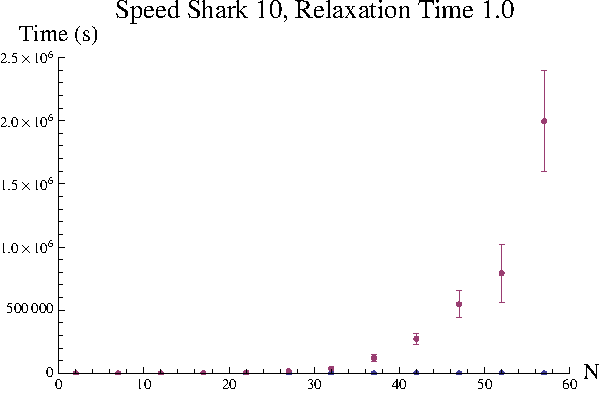
\includegraphics[width=0.45\textwidth]{shark10relaxation1.pdf}\label{fig:101}}
    \qquad
    \subfloat[]{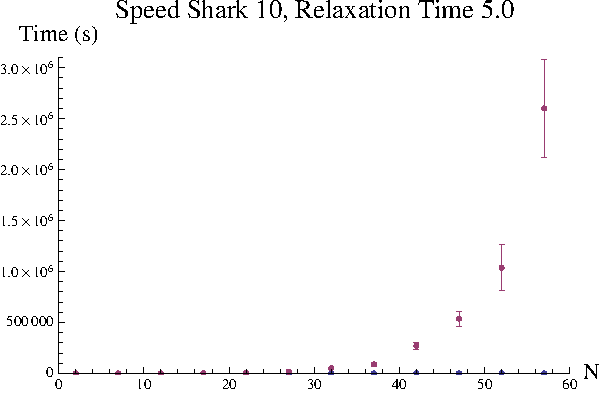
\includegraphics[width=0.45\textwidth]{shark10relaxation5.pdf}\label{fig:105}} \\
    \subfloat[]{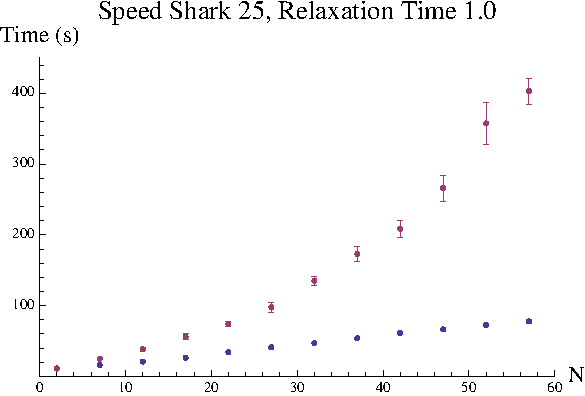
\includegraphics[width=0.45\textwidth]{shark25relaxation1.pdf}\label{fig:251}}
    \qquad
    \subfloat[]{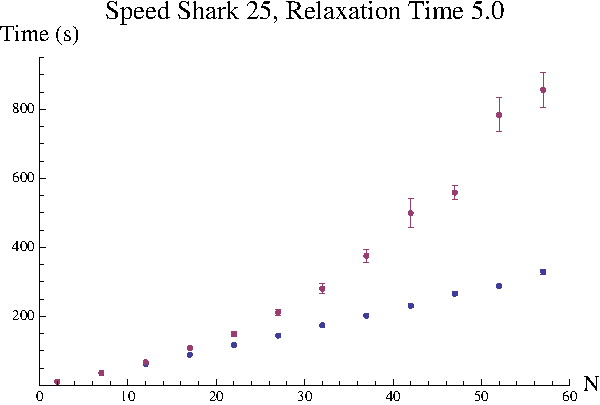
\includegraphics[width=0.45\textwidth]{shark25relaxation5.pdf}\label{fig:255}}
    \caption{The experimental results. The $x$-axis represent the number of fish in the environment ($N$). The $y$-axis denotes the time the predator required to catch all the fish. The dots represent the mean value and the bars represent the $95\%$ confidence interval. Blue denotes the original model, where fish swim in schools, while purple denotes the situation where fish swim randomly.}
    \label{fig:results}
\end{figure}


\section{Conclusions and Discussion}
\label{sec:concl}

We extended the model for the formation of fish schools introduced by Hemelrijk et. al. (2008) by adding a predator to the environment. Fish are thought to form schools in order to protect themselves from predators \cite{hemelrijk}. We tested whether the forming of a school in this model might indeed be beneficial. We found that it takes the predator a longer time to catch all the fish, when the fish swim in a random fashion rather than in a school. This result is consistent for different parameter settings (see section \ref{sec:res}). Therefore, we conclude that, in this model, the fish do not benefit from swimming in a school. 

There are some remarks to be made about the way the model is set up in this report. First of all the perception radius of the fish in the case of coherence, is set to infinity in our implementation. Hemelrijk et al. \cite{hemelrijk} used a finite perception radius to account for the limited range of vision of the fish in the school. As discussed previously we implemented it in this way because otherwise the fish school would fall apart easily when the predator is present, which would make our hypothesis untestable, since we need something that keeps resembling a stable school, even when a predator is nearby.
Moreover, our predator is not very realistic. The predator turns instantly, because the forward direction of the predator is directly updated as being the same as the direction to the nearest fish. The same essentially happens for the update of the fish position, but because the fish position is governed by forces the change is very gradually, because the forces at time $t+\Delta t$ are highly dependent on the forces at time $t$. Also the predator is assumed to have a spherical area around it, with a fish being eaten when it is in that area. This is not very realistic. An improvement would for instance be a small cone in front of the predator, indicating the eating zone. Also the predator does not rest when it is eating a fish, but rather instantaneously starts hunting the next one, which is not very realistic as well. In short, there is a lot of room for improvement on the predator.
There are also some comments to be made about the interaction between the predator and the fish. Our hypothesis was based upon the idea that the predator would get confused by all the fish in its neighborhood and hence constantly change directions, since the nearest fish changes constantly. This is however not the observed behavior in the model. An explanation is that possibly the ratio between the average distance between fish in the school and the eating radius of the predator is too small, which makes this change in direction occur less or not at all because this switching between nearest fish only occurs when the predator is close to the fish school. Also the fish school might be too static, which has the effect that the fish closest to the predator is always the same fish. Also, when the predator comes close to the fish school in our model, the dominant force becomes the fleeing force and this causes the school to become disorganized, which makes this single target chasing also more profound.
The amount of parameters used in this model is very large and the model is very sensitive to these parameters. We partly used parameters from Hemelrijk et al. \cite{hemelrijk} and partly tweaked the parameters ourselves. However it is highly likely we did not find the optimal parameter set and that there exist some parameter set which would make the school more stable and both the school and the predator behave more realistically.
Lastly, also the fact that we worked with an unbounded box instead of a tank might make a big difference, because in the case of random fish movement some fish are moving away quickly from their spawning point, and when the predator has for instance killed all the fish moving to the east of the origin, it has to swim back all the way to the west in order to chase the other fish (and which are by now very far away from the initial position). This causes our simulations for the random fish movement to run very slowly, since it takes a very long time for the predator to cover all these distances.

\begin{thebibliography}{7}
\bibitem{hemelrijk}
  C.K. Hemelrijk, H. Hildenbrandt, Self-organized shape and frontal density of fish schools, 2008, Ethology, Vol. 114, 245-254

\bibitem{kunz06}
H. Kunz, T. Z\"ublin \& C.K. Hemelrijk, On prey grouping an predator confusion in artificial fish schools, 2006, Proceedings of Tenth International Conference on Artificial Life, 365-371

\bibitem{mason}
S. Luke et al., MASON: A Multi-Agent Simulation Environment. 2005, Simulation: Transactions of the society for Modeling and Simulation International, Vol. 82(7), 517-527

\bibitem{svendsen}
J.C. Svendsen et al., Intra-school positional preference and reduced tail beat frequency in trailing positions in schooling roach under experimental conditions. , 2003, Journal Of Fish Biology, Vol. 62, 834-846

\bibitem{cullen}
S. R. Neill and J. M. Cullen, Experiments on whether schooling by their prey affects the hunting behavior of cephalopods and fish predators, 1974, Journal of Zoology, Vol 172, 549-569

\bibitem{reynolds}
C.W. Reynolds, 1987, SIGGRAPH '87: Proceedings of the 14th annual conference on Computer graphics and interactive techniques, Vol. 21(4), 25-34

\bibitem{rotmatrix}
  http://en.wikipedia.org/wiki/Rotation\_matrix\#Rotation\_matrix\_from\_axis\_and\_angle

\end{thebibliography}

\end{document}
